\documentclass{article}

\usepackage{listings}
\usepackage{graphicx}
\usepackage[hidelinks]{hyperref}

\usepackage[parfill]{parskip}

\begin{document}

\begin{titlepage}
    \centering

    \vspace*{1cm}

    % Title and subtitle are enclosed between two rules.
    \rule{\textwidth}{1pt}

    % Title
    \vspace{.7\baselineskip}
    {\huge \textbf{Dungeon Escape}}

    % Subtitle
    \vspace*{.5cm}
    {\LARGE Videojocs (VJ)}
    
    \rule{\textwidth}{1pt}

    \vspace{1cm}

    % Set this size for the remaining titlepage.
    \large

    % Authors side by side, using two minipages as a trick.
    \begin{minipage}{.5\textwidth}
        \centering
        Ignacio Folgueiras Bosque \\
        %Identification Number \textsc{654321} \\
        %{\normalsize \url{university@email.com}}
    \end{minipage}%
    \begin{minipage}{.5\textwidth}
        \centering
        Pol Forner Gomez \\
        %Identification Number \textsc{654321} \\
        %{\normalsize \url{university2@email.com}}
    \end{minipage}

    % More authors can be inserted here with additional minipages.

    \vspace{2cm}

    % Report logo.
    
\includegraphics[width=.7\textwidth]{img/fib-upc-v2-transparent.png}

    \vfill

    % University and date information at the bottom of the titlepage.
    Videojocs \\
    Facultat de Informàtica de Barcelona, UPC\\
    Año Academico: 2023-2024 \\
    Profesor: Antonio Chica \\
    5 de gener de 2024
\end{titlepage}

\tableofcontents
\newpage

\section{El juego original: Orbital Bullet}
    \begin{figure}[h]
        \centering
        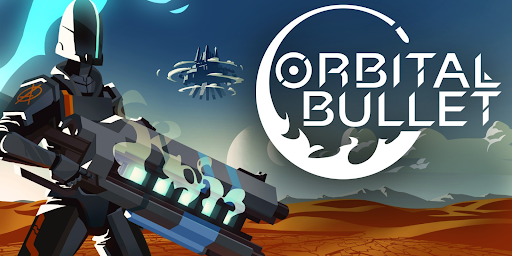
\includegraphics[width=.7\textwidth]{img/1.png}
        \caption[width=.7\textwidth]{Orbital Bullet Banner}
    \end{figure}
    Nuestro proyecto se inspira de forma directa en el juego Orbital Bullet, un juego lanzado en 2021 en acceso anticipado y al público general el 21 de marzo de 2022. 
    Fue lanzado para las plataformas PC, Switch, PlayStation 4 y Xbox One. 

\subsection{Desarollo} 

    El juego fue desarrollado por SmokeStab y publicado por Assemble Entertainment, ambas empresas independientes. 
    Aparte de la versión base tenemos la Save the World edition, la cual incluye la banda sonora original del juego y destina el 10\% de la recaudación a ONGs. 
    Su público objetivo es bastante amplio, ya que al ser un roguelike ofrece una gran variedad de formas de jugarlo, llamando a gente entre adolescentes y jóvenes adultos. 

    Saber cuanta gente ha estado involucrada en el desarollo del juego es difícil, ya que hay escasa información sobre el desarrollador SmokeStab.
    La poca información que podemos extraer a través de su Linkedin es que es un estudio con 2 - 10 empleados, es decir, muy muy pequeño.

\subsection{Ventas}
    Debido a la privacidad de sitios como Steam es difícil calcular a ciencia cierta cuántas unidades ha vendido, pero gracias a sitios como SteamSpy podemos hacer aproximaciones. 
    Según esta web, que se basa en datos recogidos del propio Steam, en total el juego ha vendido entre 20,000 y 50,000 copias. 
    Suponiendo valores no tan altos para el resto de consolas, podemos asumir que ha vendido en total unas 100.000 copias entre todas las plataformas. 
    Sabiendo que se vende a 15 euros (5 de oferta), podemos suponer que ha generado alrededor de 1.000.000€.
    Cuenta con 519 reseñas en Steam, en su mayoría positivas. Los reviewers alaban la originalidad de la idea y la rejugabilidad que proporciona.
    La mayor critica que recibe es que las opciones son algo limitadas. 

    Ha sido nominado a varios premios, quedando finalista en las nominaciones a mejor juego de estudiantes en los Independent Game Festival y mejor concepto con prototipo en los German Dev Days Awards.
\subsection{Enlaces de interes}

    Pagina oficial: \url{https://orbitalbullet.com/}

    Foro de usuarios de Steam: \url{https://steamcommunity.com/app/1167680/discussions/}

    Trailer: \url{https://www.youtube.com/watch?v=TY1vT0qD7e0}

    Gameplay: \url{https://www.youtube.com/watch?v=Z3Z4Z3Z3ZAA}

\section{Nuestro proyecto: Dungeon Escape}
    A nuestro proyecto lo hemos llamado Dungeon Escape y utiliza la mecánica 360º del juego de referencia, pero lo ambienta en un escenario de fantasía medieval. 
    Jugamos como un caballero que debe escalar los pisos para escapar de la cueva, en la cima de la cual mora un poderoso enemigo. 
    Durante su subida encontrará diversos tipos de enemigos y trampas, pero también cofres que otorgan mejoras a sus armas y aumentos a las estadísticas.

    \subsection{Instrucciones}
    Una vez iniciado el juego entraremos en la pantalla de inicio, la cual consta de 3 pantallas: 
    La pantalla de inicio, las instrucciones y los créditos.
    Desde la pantalla de inicio podemos acceder a los diferentes menús y también al juego en sí.
    En los menús, podemos navegar utilizando las siguientes teclas:
    \begin{itemize}
        \item 1 $\rightarrow$ Pantalla de inicio
        \item 2 $\rightarrow$ Instrucciones de juego 
        \item 3 $\rightarrow$ Créditos
        \item P $\rightarrow$ Empezar a jugar
    \end{itemize}
    Aqui un diagrama de flujo de la pantalla de inicio:
    \begin{figure}[h]
        \centering
        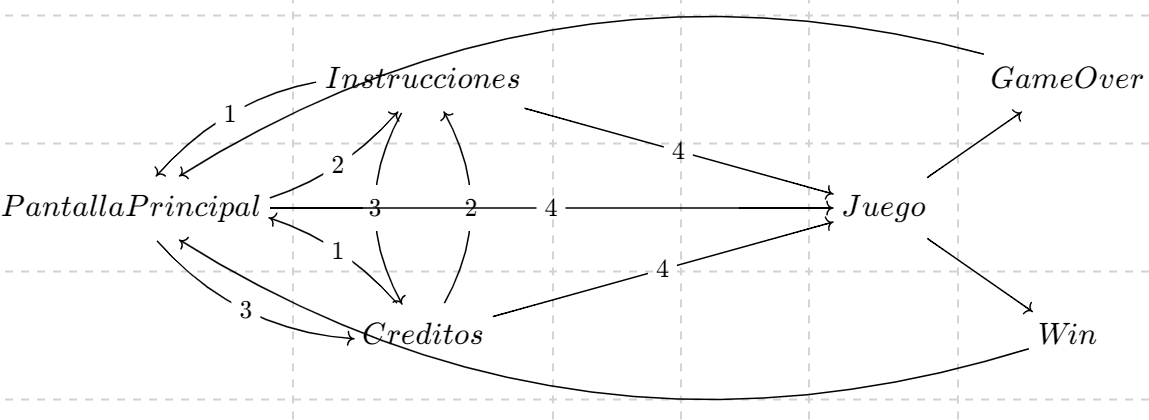
\includegraphics[width=.7\textwidth]{img/10.png}
        \caption[width=.7\textwidth]{Diagrama de ventanas}
    \end{figure}

    Durante el juego, podemos utilizar las siguientes teclas:

    \begin{itemize}
        \item P $\rightarrow$ Pausar el juego
        \item MOVIMIENTO:
        \item A$\rightarrow$ Mover hacia la izquierda
        \item D $\rightarrow$ Mover hacia la derecha
        \item W $\rightarrow$ Saltar
        \item ATACAR:
        \item 1 $\rightarrow$ Arma 1: largo alcance
        \item 2 $\rightarrow$ Arma 2: ataque cuerpo a cuerpo
        \item F $\rightarrow$ Atacar con el arma seleccionada
        \item DEBUG
        \item G $\rightarrow$ para activar del god mode
        \item Y $\rightarrow$ augmenta el daño y la HP en 100
        \item M $\rightarrow$ Maxea jugador
        \item I $\rightarrow$ Ganar HP
    \end{itemize}
\subsection{Caracteristicas implementadas}
    Respecto al enunciado, hemos implementado el movimiento básico del jugador, como moverse y saltar.
    Hemos hecho 1 fase que consta de 3 niveles, hemos añadido varios obstáculos como cajas y bariles así como pinchos, que son trampas que dañan al jugador. 
    Hemos implementado la mecánica de ir subiendo de niveles al llegar al final de cada uno. 

    También hemos añadido 2 tipos de enemigos (uno de corto alcance y otro de largo alcance), pero no hemos podido llegar a implementar sus funcionalidades. 
    También hemos añadido un jefe final, pero que tampoco hemos podido implementar sus mecánicas

    Hemos implementado los cofres, que son objetos que al ser tocados por el jugador le dan una mejora aleatoria.
\subsection{Entidades del juego}
    Aqui podreis encontrar una breve descripción de las entidades que aparecen en el juego.

\subsubsection{Jugador}
    Protagonista y personaje jugable. 
    Su objetivo es escalar la torre para escapar.
    Tiene vida y ataque los cuales pueden ser mejorados a lo largo del juego mediante los cofres.
    Cuenta con dos espadas para atacar cuerpo a cuerpo y una ballesta para atacar a distancia.
    Por falta de tiempo hemos desestimado la implementación de las armas.

    \begin{figure}[h!]
        \centering
        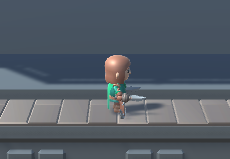
\includegraphics[width=.7\textwidth]{img/2.png}
        \caption{Modelo 3D del jugador}
    \end{figure}

\subsubsection{Pinchos}
    Trampa estática. 
    Al entrar en contacto con el jugador, le daña y desaparece. 

    \begin{figure}[h!]
        \centering
        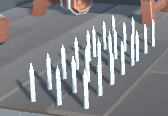
\includegraphics[width=.7\textwidth]{img/3.png}
        \caption{Modelo 3D de los pinchos}
    \end{figure}

\subsubsection{Enemigo de largo alcance: El Mago}
    Enemigo con ataques a distancia. 
    Enemigo de baja vida con la posibilidad de atacar al jugador desde lejos. 
    Por falta de tiempo hemos desestimado la implementación del mago.
    \begin{figure}[h!]
        \centering
        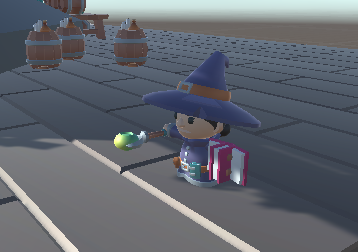
\includegraphics[width=.7\textwidth]{img/4.png}
        \caption{Modelo 3D del enemigo de largo alcance}
    \end{figure}

\subsubsection{Enemigo de corto alcance: El Barbaro}
    Enemigo con ataques a corta distancia. 
    Enemigo con buena resistencia pero limitado a solo poder atacar cuerpo a cuerpo. 
    Por falta de tiempo hemos desestimado la implementación del bárbaro.
    \begin{figure}[h!]
        \centering
        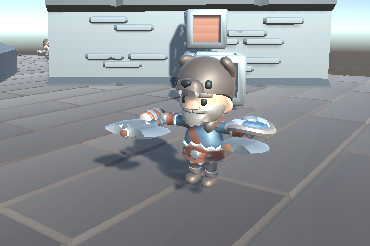
\includegraphics[width=.7\textwidth]{img/5.png}
        \caption{Modelo 3D del enemigo de corto alcance}
    \end{figure}

\subsubsection{Jefe final: El Caballero}
    Enemigo final del juego 
    Enemigo de gran tamaño con mucha vida y ataque.
    Por falta de tiempo hemos desestimado la implementación del jefe final.
    \begin{figure}[h!]
        \centering
        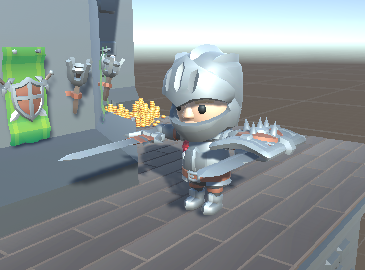
\includegraphics[width=.7\textwidth]{img/6.png}
        \caption{Modelo 3D del jefe final}
    \end{figure}

\subsubsection{Cofre}
    Recollectable.
    Cofre que puede contener diferentes power-ups, como vida, munición, armas...

    \begin{figure}[h!]
        \centering
        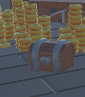
\includegraphics[width=.4\textwidth]{img/7.png}
        \caption{Modelo 3D del cofre}
    \end{figure}
\newpage 
\section{Metodología}
    La metodología de trabajo usada fue la siguiente:

    \begin{figure}[h!]
        \centering
        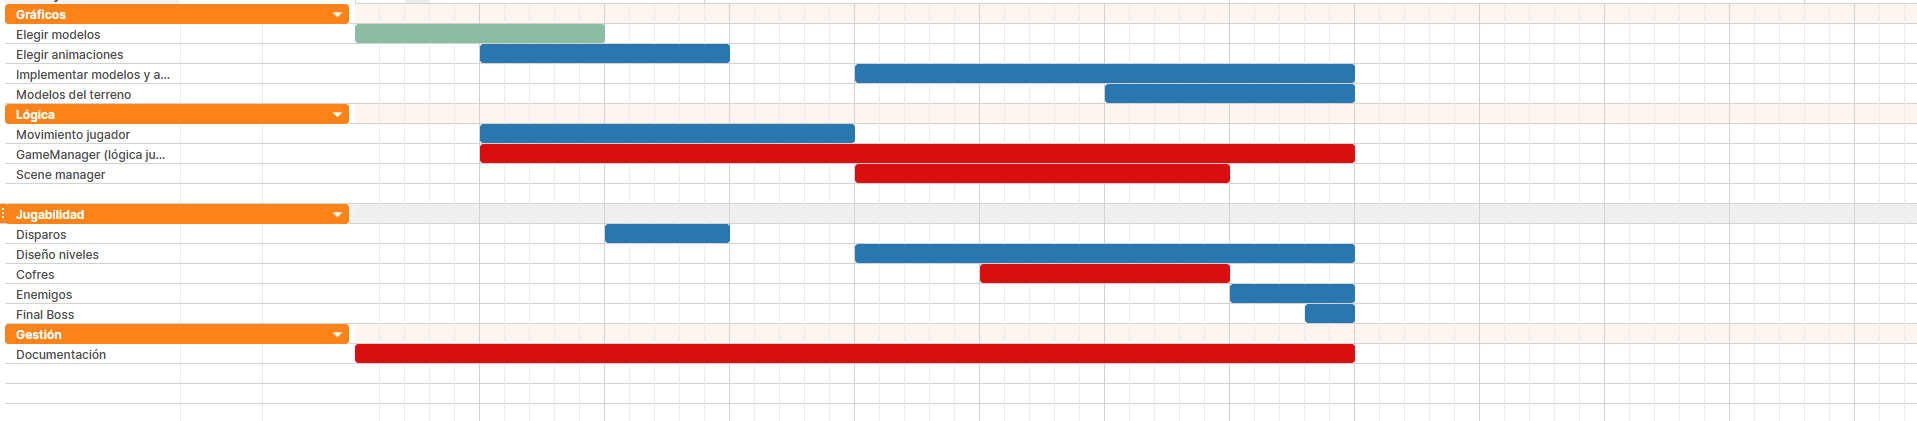
\includegraphics[width=\textwidth]{img/8.png}
        \caption{Diagrama de Gantt}
    \end{figure}

    Hicimos mucho trabajo en paralelo en distintas áreas, por lo cual no hay una gran cantidad de ramas o pulls en GitHub. 
    Aquí una captura del estado final de nuestro repositorio:
    \begin{figure}[h!]
        \centering
        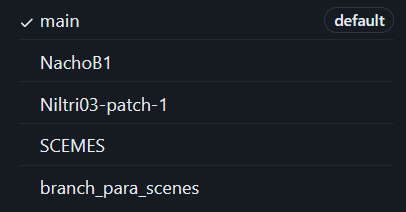
\includegraphics[width=\textwidth]{img/9.png}
        \caption{Branches en GitHub}
    \end{figure}

    Ideas descartadas:

    \begin{itemize}
        \item Al principio intentamos crear nuestros propios modelos de Voxel desde cero, y dar al juego una temática basada en Pokémon. 
                No obstante, debido a los problemas de tiempo que tuvimos los dos miembros del equipo, decidimos utilizar modelos de dominio público correspondientes a la temática medieval que tiene el juego ahora. 
        \item Respecto al sistema de mejoras, se concibió un árbol mayor. 
                Aconsejados por el profesor, esta idea acabó implementándose en la forma de aumentos al daño, vida y velocidad, ya que sería difícil implementar y equilibrar el concepto en su idea inicial en el tiempo proporcionado.
    
        \item También se descartó la idea de implementar un sistema de puntos.  
                Por problemas de tiempo, decidimos no implementar la mecánica de tener dos planos donde suceda la acción y centrarnos en implementar el resto de funciones.
    \end{itemize} 

\section{Conclusiones}
\textbf{Ignacio:}  Como conclusiones de este proyecto, me ha parecido una buena forma de practicar conceptos de niveles más avanzados de Unity, como las animaciones.
Un punto negativo es que el trabajo en remoto ha sido difícil, a causa de las limitaciones de GitHub y Unity combinados.
Como conclusiones de la asignatura, me ha parecido realmente interesante y divertida tanto la teoría como los dos proyectos prácticos, y me ha hecho ver las dificultades técnicas y los desafíos que se superan para poder crear videojuegos.

\textbf{Pol:}  Por mi parte, es cierto que he aprendido a hacer un uso básico de Unity y también de Blender.
A pesar de eso, creo ha sido un trabajo muy pesado dado a la gran cantidad de cosas a aprender para hacer un uso correcto de Unity, causando que haya hecho las cosas de forma muy “sucias”.
Creo que este trabajo sería de más provecho si tuviésemos un esqueleto del programa más completo y a partir de ahí trabajar en objetivos más concretos 

\section{Bibliografía}

\begin{itemize}

    \item “Steam: Orbital Bullet: The 360º Roguelike”: \\
    \url{https://store.steampowered.com/app/1167680/Orbital_Bullet__The_360_Roguelite/} \\
    Página del juego en la tienda virtual Steam. 
    
    \item “Steam Revenue Calculator: Orbital Bullet - The 360° rogue-lite”: \\
    \url{https://steam-revenue-calculator.com/app/1167680/orbital-bullet-the-360-rogue-lite} \\
    Página que emplea la API pública de Steam para deducir ciertos valores de los juegos en la plataforma. 

    \item “Kaykit Adventures 3D Character Pack”: \\
    \url{https://kaylousberg.itch.io/kaykit-adventurers} \\
    Página de descarga de los modelos 3D de los personajes usados.

    \item “Kaykit Dungeon 3D Asset Pack”: \\
    \url{https://kaylousberg.itch.io/kaykit-dungeon-remastered} \\
    Página de descarga de los modelos 3D usados.

    \item “Unity Forum”: \\
    \url{https://forum.unity.com/} \\
    Foro para consultar dudas sobre Unity.

    \item “Unity: Scripting API”: \\
    \url{https://docs.unity3d.com/ScriptReference} \\
    Documentación oficial de la API de Unity.

    \item “Blender Stack Exchange” : \\
    \url{https://blender.stackexchange.com} \\
    Foro para realizar consultas sobre el programa de modelado 3D Blender.

    \item “Stackoverflow” . \\
    \url{https://stackoverflow.com/} \\
    Foro de programación para dudas con C\#.
\end{itemize}

\end{document}